\begin{figure}[ht]
\centering
% Thesis-wide categorical color palette
% Usage: % Thesis-wide categorical color palette
% Usage: % Thesis-wide categorical color palette
% Usage: \input{figures/palette} in any figure file
%
% Muted primary colors -- print-friendly, visually distinct.
% Inspired by Cooper Union's red/blue primaries, softened for
% academic figures. Use palA-palC for data series in scatter
% plots, line charts, bar charts, etc.

\definecolor{palA}{HTML}{1F77B4}   % Tableau blue
\definecolor{palB}{HTML}{D62728}   % Tableau red
\definecolor{palC}{HTML}{2CA02C}   % Tableau green
 in any figure file
%
% Muted primary colors -- print-friendly, visually distinct.
% Inspired by Cooper Union's red/blue primaries, softened for
% academic figures. Use palA-palC for data series in scatter
% plots, line charts, bar charts, etc.

\definecolor{palA}{HTML}{1F77B4}   % Tableau blue
\definecolor{palB}{HTML}{D62728}   % Tableau red
\definecolor{palC}{HTML}{2CA02C}   % Tableau green
 in any figure file
%
% Muted primary colors -- print-friendly, visually distinct.
% Inspired by Cooper Union's red/blue primaries, softened for
% academic figures. Use palA-palC for data series in scatter
% plots, line charts, bar charts, etc.

\definecolor{palA}{HTML}{1F77B4}   % Tableau blue
\definecolor{palB}{HTML}{D62728}   % Tableau red
\definecolor{palC}{HTML}{2CA02C}   % Tableau green

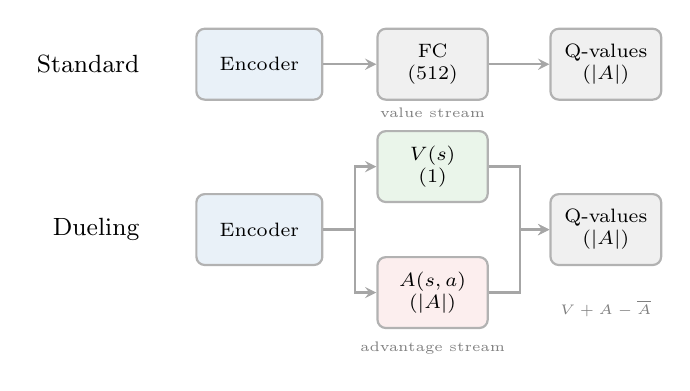
\begin{tikzpicture}[
    block/.style={draw=black!30, thick, rounded corners=3pt,
                  minimum height=0.9cm, font=\scriptsize,
                  align=center, inner sep=5pt},
    arr/.style={->, thick, >=stealth, black!35},
    lbl/.style={font=\tiny, text=black!50},
]

% --- Standard DQN (top) ---
\node[font=\small, anchor=east] at (-0.6, 1.8) {Standard};

\node[block, fill=palA!10, minimum width=1.6cm]
    (enc1) at (0.8, 1.8) {Encoder};
\node[block, fill=black!6, minimum width=1.4cm]
    (fc1) at (3.0, 1.8) {FC\\(512)};
\node[block, fill=black!6, minimum width=1.4cm]
    (q1) at (5.2, 1.8) {Q-values\\($|A|$)};

\draw[arr] (enc1) -- (fc1);
\draw[arr] (fc1) -- (q1);

% --- Dueling (bottom) ---
\node[font=\small, anchor=east] at (-0.6, -0.3) {Dueling};

\node[block, fill=palA!10, minimum width=1.6cm]
    (enc2) at (0.8, -0.3) {Encoder};

% Value stream
\node[block, fill=palC!10, minimum width=1.4cm]
    (v) at (3.0, 0.5) {$V(s)$\\(1)};

% Advantage stream
\node[block, fill=palB!8, minimum width=1.4cm]
    (a) at (3.0, -1.1) {$A(s, a)$\\($|A|$)};

% Combine
\node[block, fill=black!6, minimum width=1.4cm]
    (q2) at (5.2, -0.3) {Q-values\\($|A|$)};

\draw[arr] (enc2.east) -- ++(0.4, 0) |- (v.west);
\draw[arr] (enc2.east) -- ++(0.4, 0) |- (a.west);
\draw[arr] (v.east) -- ++(0.4, 0) |- (q2.west);
\draw[arr] (a.east) -- ++(0.4, 0) |- (q2.west);

% Stream labels
\node[lbl, above=1pt] at (v.north) {value stream};
\node[lbl, below=1pt] at (a.south) {advantage stream};

% Combine label
\node[lbl] at (5.2, -1.3)
    {$V + A - \overline{A}$};

\end{tikzpicture}
\caption{Dueling architecture. The encoder output splits into a
  value stream $V(s)$ and an advantage stream $A(s, a)$, which
  recombine to produce Q-values.}
\label{fig:dueling-architecture}
\end{figure}
